\documentclass[]{article}
\usepackage{lmodern}
\usepackage{amssymb,amsmath}
\usepackage{ifxetex,ifluatex}
\usepackage{fixltx2e} % provides \textsubscript
\ifnum 0\ifxetex 1\fi\ifluatex 1\fi=0 % if pdftex
  \usepackage[T1]{fontenc}
  \usepackage[utf8]{inputenc}
\else % if luatex or xelatex
  \ifxetex
    \usepackage{mathspec}
  \else
    \usepackage{fontspec}
  \fi
  \defaultfontfeatures{Ligatures=TeX,Scale=MatchLowercase}
\fi
% use upquote if available, for straight quotes in verbatim environments
\IfFileExists{upquote.sty}{\usepackage{upquote}}{}
% use microtype if available
\IfFileExists{microtype.sty}{%
\usepackage{microtype}
\UseMicrotypeSet[protrusion]{basicmath} % disable protrusion for tt fonts
}{}
\usepackage[margin=1in]{geometry}
\usepackage{hyperref}
\hypersetup{unicode=true,
            pdftitle={COMPSCIX 415.2 Homework 8},
            pdfauthor={Bryan Hee},
            pdfborder={0 0 0},
            breaklinks=true}
\urlstyle{same}  % don't use monospace font for urls
\usepackage{color}
\usepackage{fancyvrb}
\newcommand{\VerbBar}{|}
\newcommand{\VERB}{\Verb[commandchars=\\\{\}]}
\DefineVerbatimEnvironment{Highlighting}{Verbatim}{commandchars=\\\{\}}
% Add ',fontsize=\small' for more characters per line
\usepackage{framed}
\definecolor{shadecolor}{RGB}{248,248,248}
\newenvironment{Shaded}{\begin{snugshade}}{\end{snugshade}}
\newcommand{\KeywordTok}[1]{\textcolor[rgb]{0.13,0.29,0.53}{\textbf{#1}}}
\newcommand{\DataTypeTok}[1]{\textcolor[rgb]{0.13,0.29,0.53}{#1}}
\newcommand{\DecValTok}[1]{\textcolor[rgb]{0.00,0.00,0.81}{#1}}
\newcommand{\BaseNTok}[1]{\textcolor[rgb]{0.00,0.00,0.81}{#1}}
\newcommand{\FloatTok}[1]{\textcolor[rgb]{0.00,0.00,0.81}{#1}}
\newcommand{\ConstantTok}[1]{\textcolor[rgb]{0.00,0.00,0.00}{#1}}
\newcommand{\CharTok}[1]{\textcolor[rgb]{0.31,0.60,0.02}{#1}}
\newcommand{\SpecialCharTok}[1]{\textcolor[rgb]{0.00,0.00,0.00}{#1}}
\newcommand{\StringTok}[1]{\textcolor[rgb]{0.31,0.60,0.02}{#1}}
\newcommand{\VerbatimStringTok}[1]{\textcolor[rgb]{0.31,0.60,0.02}{#1}}
\newcommand{\SpecialStringTok}[1]{\textcolor[rgb]{0.31,0.60,0.02}{#1}}
\newcommand{\ImportTok}[1]{#1}
\newcommand{\CommentTok}[1]{\textcolor[rgb]{0.56,0.35,0.01}{\textit{#1}}}
\newcommand{\DocumentationTok}[1]{\textcolor[rgb]{0.56,0.35,0.01}{\textbf{\textit{#1}}}}
\newcommand{\AnnotationTok}[1]{\textcolor[rgb]{0.56,0.35,0.01}{\textbf{\textit{#1}}}}
\newcommand{\CommentVarTok}[1]{\textcolor[rgb]{0.56,0.35,0.01}{\textbf{\textit{#1}}}}
\newcommand{\OtherTok}[1]{\textcolor[rgb]{0.56,0.35,0.01}{#1}}
\newcommand{\FunctionTok}[1]{\textcolor[rgb]{0.00,0.00,0.00}{#1}}
\newcommand{\VariableTok}[1]{\textcolor[rgb]{0.00,0.00,0.00}{#1}}
\newcommand{\ControlFlowTok}[1]{\textcolor[rgb]{0.13,0.29,0.53}{\textbf{#1}}}
\newcommand{\OperatorTok}[1]{\textcolor[rgb]{0.81,0.36,0.00}{\textbf{#1}}}
\newcommand{\BuiltInTok}[1]{#1}
\newcommand{\ExtensionTok}[1]{#1}
\newcommand{\PreprocessorTok}[1]{\textcolor[rgb]{0.56,0.35,0.01}{\textit{#1}}}
\newcommand{\AttributeTok}[1]{\textcolor[rgb]{0.77,0.63,0.00}{#1}}
\newcommand{\RegionMarkerTok}[1]{#1}
\newcommand{\InformationTok}[1]{\textcolor[rgb]{0.56,0.35,0.01}{\textbf{\textit{#1}}}}
\newcommand{\WarningTok}[1]{\textcolor[rgb]{0.56,0.35,0.01}{\textbf{\textit{#1}}}}
\newcommand{\AlertTok}[1]{\textcolor[rgb]{0.94,0.16,0.16}{#1}}
\newcommand{\ErrorTok}[1]{\textcolor[rgb]{0.64,0.00,0.00}{\textbf{#1}}}
\newcommand{\NormalTok}[1]{#1}
\usepackage{graphicx,grffile}
\makeatletter
\def\maxwidth{\ifdim\Gin@nat@width>\linewidth\linewidth\else\Gin@nat@width\fi}
\def\maxheight{\ifdim\Gin@nat@height>\textheight\textheight\else\Gin@nat@height\fi}
\makeatother
% Scale images if necessary, so that they will not overflow the page
% margins by default, and it is still possible to overwrite the defaults
% using explicit options in \includegraphics[width, height, ...]{}
\setkeys{Gin}{width=\maxwidth,height=\maxheight,keepaspectratio}
\IfFileExists{parskip.sty}{%
\usepackage{parskip}
}{% else
\setlength{\parindent}{0pt}
\setlength{\parskip}{6pt plus 2pt minus 1pt}
}
\setlength{\emergencystretch}{3em}  % prevent overfull lines
\providecommand{\tightlist}{%
  \setlength{\itemsep}{0pt}\setlength{\parskip}{0pt}}
\setcounter{secnumdepth}{0}
% Redefines (sub)paragraphs to behave more like sections
\ifx\paragraph\undefined\else
\let\oldparagraph\paragraph
\renewcommand{\paragraph}[1]{\oldparagraph{#1}\mbox{}}
\fi
\ifx\subparagraph\undefined\else
\let\oldsubparagraph\subparagraph
\renewcommand{\subparagraph}[1]{\oldsubparagraph{#1}\mbox{}}
\fi

%%% Use protect on footnotes to avoid problems with footnotes in titles
\let\rmarkdownfootnote\footnote%
\def\footnote{\protect\rmarkdownfootnote}

%%% Change title format to be more compact
\usepackage{titling}

% Create subtitle command for use in maketitle
\newcommand{\subtitle}[1]{
  \posttitle{
    \begin{center}\large#1\end{center}
    }
}

\setlength{\droptitle}{-2em}
  \title{COMPSCIX 415.2 Homework 8}
  \pretitle{\vspace{\droptitle}\centering\huge}
  \posttitle{\par}
  \author{Bryan Hee}
  \preauthor{\centering\large\emph}
  \postauthor{\par}
  \predate{\centering\large\emph}
  \postdate{\par}
  \date{March 26, 2018}


\begin{document}
\maketitle

\subsubsection{Exercise 1}\label{exercise-1}

There are 891 observations or people and 12 variables/columns in the
Titanic training dataset.

\begin{Shaded}
\begin{Highlighting}[]
\NormalTok{Titanic_kaggle <-}\StringTok{ }\KeywordTok{read.csv}\NormalTok{(}\StringTok{"C:/Users/BryanHee/OneDrive - stok LLC/Intro to Data Science/HW Assignments/Assignment 8/train.csv"}\NormalTok{, }\DataTypeTok{sep =} \StringTok{","}\NormalTok{)}
\NormalTok{Titanic_kaggle <-}\StringTok{ }\KeywordTok{transform}\NormalTok{(Titanic_kaggle, }\DataTypeTok{Survived =} \KeywordTok{as.factor}\NormalTok{(Survived))}
\KeywordTok{glimpse}\NormalTok{(Titanic_kaggle)}
\end{Highlighting}
\end{Shaded}

\begin{verbatim}
## Observations: 891
## Variables: 12
## $ PassengerId <int> 1, 2, 3, 4, 5, 6, 7, 8, 9, 10, 11, 12, 13, 14, 15,...
## $ Survived    <fct> 0, 1, 1, 1, 0, 0, 0, 0, 1, 1, 1, 1, 0, 0, 0, 1, 0,...
## $ Pclass      <int> 3, 1, 3, 1, 3, 3, 1, 3, 3, 2, 3, 1, 3, 3, 3, 2, 3,...
## $ Name        <fct> Braund, Mr. Owen Harris, Cumings, Mrs. John Bradle...
## $ Sex         <fct> male, female, female, female, male, male, male, ma...
## $ Age         <dbl> 22, 38, 26, 35, 35, NA, 54, 2, 27, 14, 4, 58, 20, ...
## $ SibSp       <int> 1, 1, 0, 1, 0, 0, 0, 3, 0, 1, 1, 0, 0, 1, 0, 0, 4,...
## $ Parch       <int> 0, 0, 0, 0, 0, 0, 0, 1, 2, 0, 1, 0, 0, 5, 0, 0, 1,...
## $ Ticket      <fct> A/5 21171, PC 17599, STON/O2. 3101282, 113803, 373...
## $ Fare        <dbl> 7.2500, 71.2833, 7.9250, 53.1000, 8.0500, 8.4583, ...
## $ Cabin       <fct> , C85, , C123, , , E46, , , , G6, C103, , , , , , ...
## $ Embarked    <fct> S, C, S, S, S, Q, S, S, S, C, S, S, S, S, S, S, Q,...
\end{verbatim}

\begin{Shaded}
\begin{Highlighting}[]
\NormalTok{Titanic_kaggle }\OperatorTok
\StringTok{  }\KeywordTok{group_by}\NormalTok{(Survived) }\OperatorTok
\StringTok{  }\KeywordTok{summarise}\NormalTok{(}\DataTypeTok{count =} \KeywordTok{n}\NormalTok{())}
\end{Highlighting}
\end{Shaded}

\begin{verbatim}
## # A tibble: 2 x 2
##   Survived count
##   <fct>    <int>
## 1 0          549
## 2 1          342
\end{verbatim}

\subsubsection{Exercise 2}\label{exercise-2}

\begin{Shaded}
\begin{Highlighting}[]
\KeywordTok{set.seed}\NormalTok{(}\DecValTok{29283}\NormalTok{)}

\NormalTok{Titanic_train <-}\StringTok{ }\NormalTok{Titanic_kaggle }\OperatorTok\StringTok{ }\KeywordTok{sample_frac}\NormalTok{(}\FloatTok{0.7}\NormalTok{)}
\NormalTok{Titanic_test <-}\StringTok{ }\NormalTok{Titanic_kaggle }\OperatorTok\StringTok{ }\KeywordTok{filter}\NormalTok{(}\OperatorTok{!}\NormalTok{(Titanic_kaggle}\OperatorTok{$}\NormalTok{PassengerId }\OperatorTok\StringTok{ }\NormalTok{Titanic_train}\OperatorTok{$}\NormalTok{PassengerId))}
\end{Highlighting}
\end{Shaded}

\subsubsection{Exercise 3}\label{exercise-3}

Using a logistic regression model, Survived is predicted based off of
the attributes Pclass, Sex and Fare.

Based off of the broom function, tidy, we are able to see the estimates,
std.error, statistics, and p.values of the model inputs. The estimate
related to class tells us that as the Pclass value goes up by one
(i.e.~going from middle class to lower class), the odds of survival
drops by \textasciitilde{}0.88. The odds are related to the probability.
The coefficient associated with sex is intepretted as: males' odds of
survival is 2.8 less than women. The fare estimate predicts that as the
fare goes up by \$1, the odds of survival go up by
\textasciitilde{}0.002.

Based off of a 0.5 p-value cutoff, all features are significant. Fare is
extremely close to the cutoff though.

\begin{Shaded}
\begin{Highlighting}[]
\NormalTok{mod_}\DecValTok{1}\NormalTok{ <-}\StringTok{ }\KeywordTok{glm}\NormalTok{(Survived }\OperatorTok{~}\StringTok{ }\NormalTok{Pclass }\OperatorTok{+}\StringTok{ }\NormalTok{Sex }\OperatorTok{+}\StringTok{ }\NormalTok{Fare, }\DataTypeTok{data =}\NormalTok{ Titanic_train, }\DataTypeTok{family =} \StringTok{'binomial'}\NormalTok{)}
\KeywordTok{tidy}\NormalTok{(mod_}\DecValTok{1}\NormalTok{)}
\end{Highlighting}
\end{Shaded}

\begin{verbatim}
##          term     estimate   std.error   statistic      p.value
## 1 (Intercept)  3.158129368 0.430541964   7.3352417 2.213217e-13
## 2      Pclass -0.875841345 0.145107088  -6.0358274 1.581502e-09
## 3     Sexmale -2.840421241 0.228239516 -12.4449144 1.490440e-35
## 4        Fare  0.001846965 0.002290049   0.8065179 4.199443e-01
\end{verbatim}

\subsubsection{Exercise 4}\label{exercise-4}

One path a Titanic passenger might take down the tree: A female
passenger with a class proxy number greater than or equal to 2.5, and a
fare value less than \$23.7 but greater than or equal to 15 dollars has
a 75\% probability of survival based off of the training dataset.

Something that surprises me about the results of the tree, was that the
node with the second lowest probability of survival was lower class
women who had paid a lot for their fare. Also, most lower class women
who paid less than 7.90 dollars survived. However, most lower class
women who paid a little more (\textgreater{}\$7.90 but \textless{} 15
dollars) died.

\begin{Shaded}
\begin{Highlighting}[]
\NormalTok{tree_mod <-}\StringTok{ }\KeywordTok{rpart}\NormalTok{(Survived }\OperatorTok{~}\StringTok{ }\NormalTok{Pclass }\OperatorTok{+}\StringTok{ }\NormalTok{Sex }\OperatorTok{+}\StringTok{ }\NormalTok{Fare, }\DataTypeTok{data =}\NormalTok{ Titanic_train)}
\NormalTok{tree_mod}
\end{Highlighting}
\end{Shaded}

\begin{verbatim}
## n= 624 
## 
## node), split, n, loss, yval, (yprob)
##       * denotes terminal node
## 
##  1) root 624 237 0 (0.62019231 0.37980769)  
##    2) Sex=male 411  73 0 (0.82238443 0.17761557) *
##    3) Sex=female 213  49 1 (0.23004695 0.76995305)  
##      6) Pclass>=2.5 93  45 1 (0.48387097 0.51612903)  
##       12) Fare>=23.7 17   2 0 (0.88235294 0.11764706) *
##       13) Fare< 23.7 76  30 1 (0.39473684 0.60526316)  
##         26) Fare>=7.8875 47  22 1 (0.46808511 0.53191489)  
##           52) Fare< 15 27  10 0 (0.62962963 0.37037037) *
##           53) Fare>=15 20   5 1 (0.25000000 0.75000000) *
##         27) Fare< 7.8875 29   8 1 (0.27586207 0.72413793) *
##      7) Pclass< 2.5 120   4 1 (0.03333333 0.96666667) *
\end{verbatim}

\begin{Shaded}
\begin{Highlighting}[]
\KeywordTok{plot}\NormalTok{(}\KeywordTok{as.party}\NormalTok{(tree_mod))}
\end{Highlighting}
\end{Shaded}

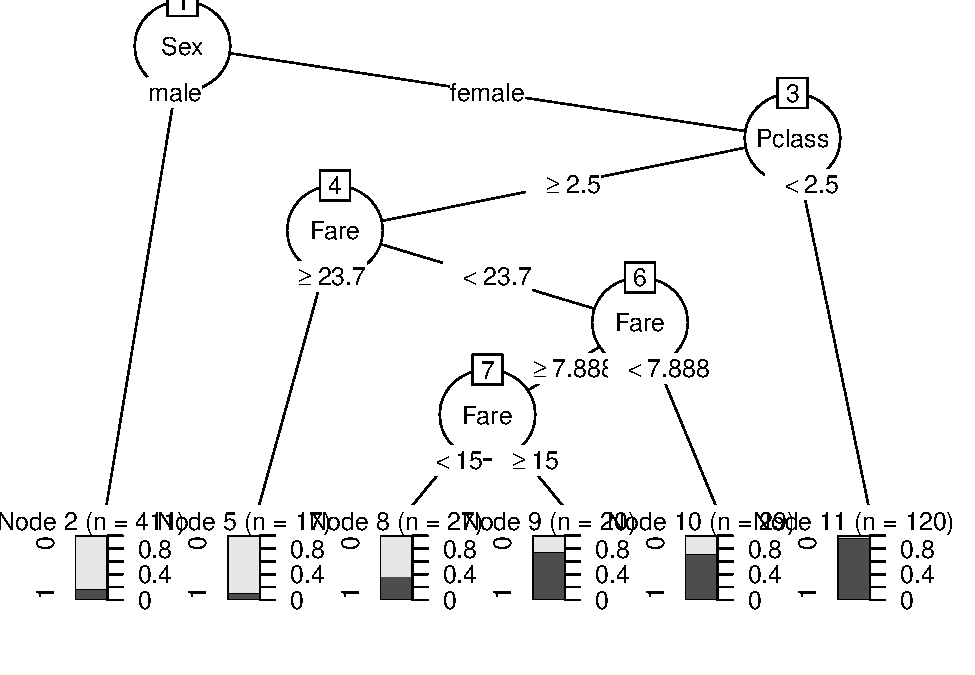
\includegraphics{homework_8_Hee_Bryan_files/figure-latex/unnamed-chunk-3-1.pdf}

\subsubsection{Exercise 5}\label{exercise-5}

For the following code, i chose to use the train dataset to then inform
the predictions on the test dataset. This code differed slightly from
what was provided on the homework handout.

\begin{Shaded}
\begin{Highlighting}[]
\NormalTok{mod_}\DecValTok{2}\NormalTok{ <-}\StringTok{ }\KeywordTok{glm}\NormalTok{(Survived }\OperatorTok{~}\StringTok{ }\NormalTok{Pclass }\OperatorTok{+}\StringTok{ }\NormalTok{Sex }\OperatorTok{+}\StringTok{ }\NormalTok{Fare, }\DataTypeTok{data =}\NormalTok{ Titanic_train, }\DataTypeTok{family =} \StringTok{'binomial'}\NormalTok{)}
\KeywordTok{tidy}\NormalTok{(mod_}\DecValTok{2}\NormalTok{)}
\end{Highlighting}
\end{Shaded}

\begin{verbatim}
##          term     estimate   std.error   statistic      p.value
## 1 (Intercept)  3.158129368 0.430541964   7.3352417 2.213217e-13
## 2      Pclass -0.875841345 0.145107088  -6.0358274 1.581502e-09
## 3     Sexmale -2.840421241 0.228239516 -12.4449144 1.490440e-35
## 4        Fare  0.001846965 0.002290049   0.8065179 4.199443e-01
\end{verbatim}

\begin{Shaded}
\begin{Highlighting}[]
\NormalTok{test_logit <-}\StringTok{ }\KeywordTok{predict}\NormalTok{(mod_}\DecValTok{2}\NormalTok{, }\DataTypeTok{newdata =}\NormalTok{ Titanic_test, }\DataTypeTok{type =} \StringTok{'response'}\NormalTok{)}

\NormalTok{tree_mod2 <-}\StringTok{ }\KeywordTok{rpart}\NormalTok{(Survived }\OperatorTok{~}\StringTok{ }\NormalTok{Pclass }\OperatorTok{+}\StringTok{ }\NormalTok{Sex }\OperatorTok{+}\StringTok{ }\NormalTok{Fare, }\DataTypeTok{data =}\NormalTok{ Titanic_train)}
\NormalTok{test_tree <-}\StringTok{ }\KeywordTok{predict}\NormalTok{(tree_mod2, }\DataTypeTok{newdata =}\NormalTok{ Titanic_test)[,}\DecValTok{2}\NormalTok{]}
\end{Highlighting}
\end{Shaded}

\begin{Shaded}
\begin{Highlighting}[]
\NormalTok{pred_logit <-}\StringTok{ }\KeywordTok{prediction}\NormalTok{(}\DataTypeTok{predictions =}\NormalTok{ test_logit, }\DataTypeTok{labels =}\NormalTok{ Titanic_test}\OperatorTok{$}\NormalTok{Survived)}
\NormalTok{pred_tree <-}\StringTok{ }\KeywordTok{prediction}\NormalTok{(}\DataTypeTok{predictions =}\NormalTok{ test_tree, }\DataTypeTok{labels =}\NormalTok{ Titanic_test}\OperatorTok{$}\NormalTok{Survived)}

\NormalTok{perf_logit <-}\StringTok{ }\KeywordTok{performance}\NormalTok{(pred_logit, }\DataTypeTok{measure =} \StringTok{'tpr'}\NormalTok{, }\DataTypeTok{x.measure =} \StringTok{'fpr'}\NormalTok{)}
\NormalTok{perf_logit_tbl <-}\StringTok{ }\KeywordTok{tibble}\NormalTok{(perf_logit}\OperatorTok{@}\NormalTok{x.values[[}\DecValTok{1}\NormalTok{]], perf_logit}\OperatorTok{@}\NormalTok{y.values[[}\DecValTok{1}\NormalTok{]])}
\KeywordTok{names}\NormalTok{(perf_logit_tbl) <-}\StringTok{ }\KeywordTok{c}\NormalTok{(}\StringTok{'fpr'}\NormalTok{, }\StringTok{'tpr'}\NormalTok{)}

\NormalTok{perf_tree <-}\StringTok{ }\KeywordTok{performance}\NormalTok{(pred_tree, }\DataTypeTok{measure =} \StringTok{'tpr'}\NormalTok{, }\DataTypeTok{x.measure =} \StringTok{'fpr'}\NormalTok{)}
\NormalTok{perf_tree_tbl <-}\StringTok{ }\KeywordTok{tibble}\NormalTok{(perf_tree}\OperatorTok{@}\NormalTok{x.values[[}\DecValTok{1}\NormalTok{]], perf_tree}\OperatorTok{@}\NormalTok{y.values[[}\DecValTok{1}\NormalTok{]])}
\KeywordTok{names}\NormalTok{(perf_tree_tbl) <-}\StringTok{ }\KeywordTok{c}\NormalTok{(}\StringTok{'fpr'}\NormalTok{, }\StringTok{'tpr'}\NormalTok{)}

\NormalTok{plot_roc <-}\StringTok{ }\ControlFlowTok{function}\NormalTok{(perf_tbl) \{}
\NormalTok{  p <-}\StringTok{ }\KeywordTok{ggplot}\NormalTok{(}\DataTypeTok{data =}\NormalTok{ perf_tbl, }\KeywordTok{aes}\NormalTok{(}\DataTypeTok{x =}\NormalTok{ fpr, }\DataTypeTok{y =}\NormalTok{ tpr)) }\OperatorTok{+}
\StringTok{  }\KeywordTok{geom_line}\NormalTok{(}\DataTypeTok{color =} \StringTok{'blue'}\NormalTok{) }\OperatorTok{+}
\StringTok{  }\KeywordTok{geom_abline}\NormalTok{(}\DataTypeTok{intercept =} \DecValTok{0}\NormalTok{, }\DataTypeTok{slope =} \DecValTok{1}\NormalTok{, }\DataTypeTok{lty =} \DecValTok{3}\NormalTok{) }\OperatorTok{+}
\StringTok{  }\KeywordTok{labs}\NormalTok{(}\DataTypeTok{x =} \StringTok{'False positive rate'}\NormalTok{, }\DataTypeTok{y =} \StringTok{'True positive rate'}\NormalTok{) }\OperatorTok{+}
\StringTok{  }\KeywordTok{theme_bw}\NormalTok{()}
  \KeywordTok{return}\NormalTok{(p)}
\NormalTok{\}}

\KeywordTok{plot_roc}\NormalTok{(perf_logit_tbl)}
\end{Highlighting}
\end{Shaded}

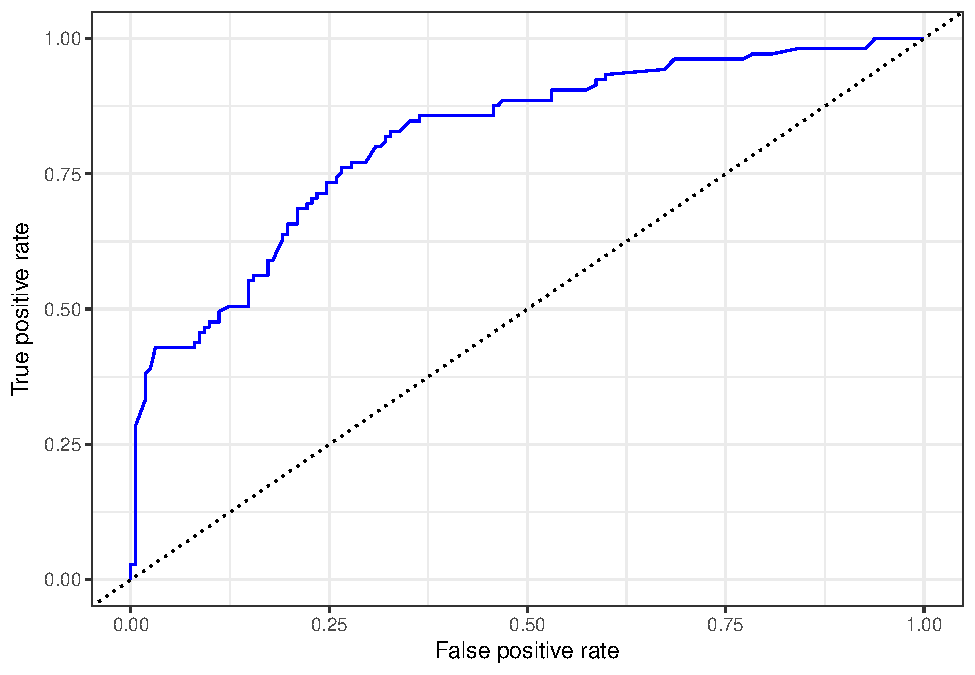
\includegraphics{./tex2pdf.13052/c121bc234d5332f335887d3567b0fa306b099364.pdf}

\begin{Shaded}
\begin{Highlighting}[]
\KeywordTok{plot_roc}\NormalTok{(perf_tree_tbl)}
\end{Highlighting}
\end{Shaded}

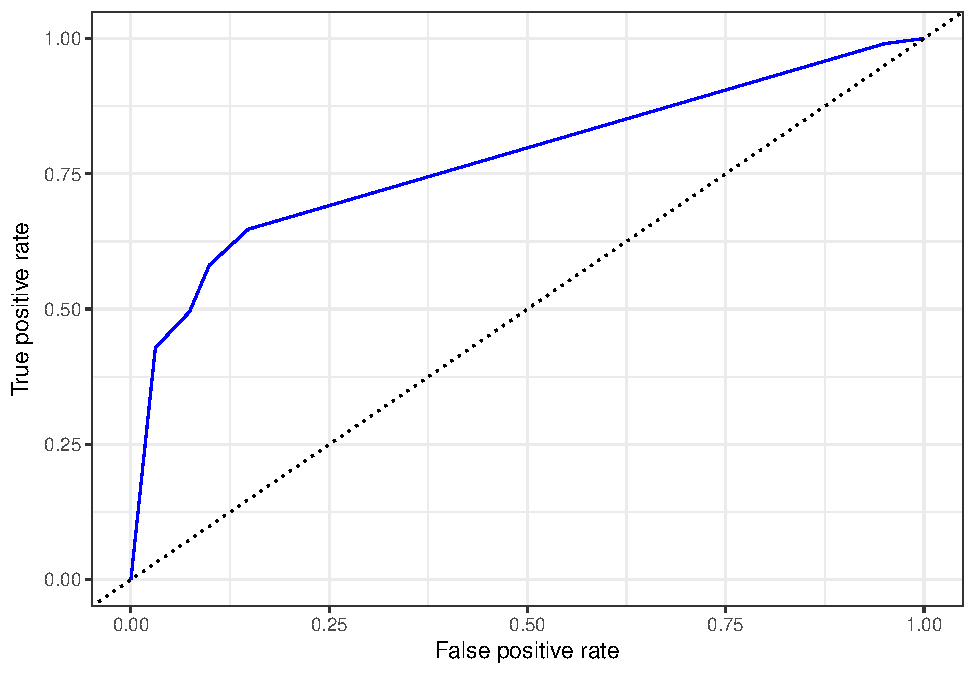
\includegraphics{./tex2pdf.13052/5d97af7ca217d219a91bd628217bc3c75190493c.pdf}

Based off of the area under the curve, AUC, values both models seem to
be performing decently well. Anything greater than 0.5 is better than a
chance guess. The Logistic model is actually performing better than the
classification tree, which was surprising to me. These models could
probably be improved by swapping out a feature for fare.

\begin{Shaded}
\begin{Highlighting}[]
\NormalTok{auc_logit <-}\StringTok{ }\KeywordTok{performance}\NormalTok{(}\DataTypeTok{prediction.obj =}\NormalTok{ pred_logit, }\DataTypeTok{measure =} \StringTok{"auc"}\NormalTok{)}
\NormalTok{auc_tree <-}\StringTok{ }\KeywordTok{performance}\NormalTok{(}\DataTypeTok{prediction.obj =}\NormalTok{ pred_tree, }\DataTypeTok{measure =} \StringTok{"auc"}\NormalTok{)}

\CommentTok{# extract the AUC value}
\NormalTok{auc_logit}\OperatorTok{@}\NormalTok{y.values[[}\DecValTok{1}\NormalTok{]]}
\end{Highlighting}
\end{Shaded}

\begin{verbatim}
## [1] 0.8147854
\end{verbatim}

\begin{Shaded}
\begin{Highlighting}[]
\NormalTok{auc_tree}\OperatorTok{@}\NormalTok{y.values[[}\DecValTok{1}\NormalTok{]]}
\end{Highlighting}
\end{Shaded}

\begin{verbatim}
## [1] 0.776602
\end{verbatim}

\begin{Shaded}
\begin{Highlighting}[]
\NormalTok{Titanic_test }\OperatorTok
\StringTok{  }\KeywordTok{mutate}\NormalTok{(}\DataTypeTok{pred_logit =}\NormalTok{ test_logit,}
         \DataTypeTok{pred_tree =}\NormalTok{ test_tree) ->}\StringTok{ }\NormalTok{Titanic_test}

\NormalTok{cutoff =}\StringTok{ }\FloatTok{0.3}
\NormalTok{Titanic_test }\OperatorTok
\StringTok{  }\KeywordTok{mutate}\NormalTok{(}\DataTypeTok{logit =} \KeywordTok{case_when}\NormalTok{(pred_logit }\OperatorTok{>=}\StringTok{ }\NormalTok{cutoff }\OperatorTok{~}\StringTok{ "yes"}\NormalTok{,}
\NormalTok{                   pred_logit }\OperatorTok{<}\StringTok{ }\NormalTok{cutoff }\OperatorTok{~}\StringTok{ "no"}\NormalTok{), }
         \DataTypeTok{tree =}  \KeywordTok{case_when}\NormalTok{(pred_tree }\OperatorTok{>=}\StringTok{ }\NormalTok{cutoff }\OperatorTok{~}\StringTok{ "yes"}\NormalTok{,}
\NormalTok{                           pred_tree }\OperatorTok{<}\StringTok{ }\NormalTok{cutoff }\OperatorTok{~}\StringTok{ "no"}\NormalTok{)) ->}\StringTok{ }\NormalTok{Titanic_test}


\NormalTok{Titanic_test }\OperatorTok\StringTok{ }\KeywordTok{count}\NormalTok{(logit, Survived) }\OperatorTok\StringTok{ }\KeywordTok{spread}\NormalTok{(Survived, n)}
\end{Highlighting}
\end{Shaded}

\begin{verbatim}
## # A tibble: 2 x 3
##   logit   `0`   `1`
## * <chr> <int> <int>
## 1 no      112    21
## 2 yes      50    84
\end{verbatim}

\begin{Shaded}
\begin{Highlighting}[]
\NormalTok{Titanic_test }\OperatorTok\StringTok{ }\KeywordTok{count}\NormalTok{(tree, Survived) }\OperatorTok\StringTok{ }\KeywordTok{spread}\NormalTok{(Survived, n)}
\end{Highlighting}
\end{Shaded}

\begin{verbatim}
## # A tibble: 2 x 3
##   tree    `0`   `1`
## * <chr> <int> <int>
## 1 no      138    37
## 2 yes      24    68
\end{verbatim}

\subsubsection{Exercise 6}\label{exercise-6}

\begin{Shaded}
\begin{Highlighting}[]
\NormalTok{Titanic_train }\OperatorTok\StringTok{ }
\StringTok{  }\KeywordTok{filter}\NormalTok{(}\OperatorTok{!}\KeywordTok{is.na}\NormalTok{(Titanic_train}\OperatorTok{$}\NormalTok{Age)) ->}\StringTok{ }\NormalTok{Titanic_train2}
\NormalTok{Titanic_test }\OperatorTok
\StringTok{  }\KeywordTok{filter}\NormalTok{(}\OperatorTok{!}\KeywordTok{is.na}\NormalTok{(Titanic_test}\OperatorTok{$}\NormalTok{Age)) ->}\StringTok{ }\NormalTok{Titanic_test2}


\NormalTok{logit_mod6 <-}\StringTok{ }\KeywordTok{glm}\NormalTok{(Survived }\OperatorTok{~}\StringTok{ }\NormalTok{Pclass }\OperatorTok{+}\StringTok{ }\NormalTok{Sex }\OperatorTok{+}\StringTok{ }\NormalTok{Age, }\DataTypeTok{data =}\NormalTok{ Titanic_train2, }\DataTypeTok{family =} \StringTok{'binomial'}\NormalTok{)}
\KeywordTok{tidy}\NormalTok{(logit_mod6)}
\end{Highlighting}
\end{Shaded}

\begin{verbatim}
##          term    estimate   std.error  statistic      p.value
## 1 (Intercept)  4.69299343 0.602182541   7.793307 6.527774e-15
## 2      Pclass -1.15981402 0.165626890  -7.002571 2.513078e-12
## 3     Sexmale -2.66313941 0.247843014 -10.745267 6.238101e-27
## 4         Age -0.03199468 0.009636951  -3.320001 9.001728e-04
\end{verbatim}

\begin{Shaded}
\begin{Highlighting}[]
\NormalTok{test_logit6 <-}\StringTok{ }\KeywordTok{predict}\NormalTok{(logit_mod6, }\DataTypeTok{newdata =}\NormalTok{ Titanic_test2, }\DataTypeTok{type =} \StringTok{'response'}\NormalTok{)}

\NormalTok{tree_mod6 <-}\StringTok{ }\KeywordTok{rpart}\NormalTok{(Survived }\OperatorTok{~}\StringTok{ }\NormalTok{Pclass }\OperatorTok{+}\StringTok{ }\NormalTok{Sex }\OperatorTok{+}\StringTok{ }\NormalTok{Age, }\DataTypeTok{data =}\NormalTok{ Titanic_train2)}
\NormalTok{tree_mod6}
\end{Highlighting}
\end{Shaded}

\begin{verbatim}
## n= 506 
## 
## node), split, n, loss, yval, (yprob)
##       * denotes terminal node
## 
##  1) root 506 205 0 (0.59486166 0.40513834)  
##    2) Sex=male 322  62 0 (0.80745342 0.19254658) *
##    3) Sex=female 184  41 1 (0.22282609 0.77717391)  
##      6) Pclass>=2.5 70  33 0 (0.52857143 0.47142857)  
##       12) Age>=27.5 19   5 0 (0.73684211 0.26315789) *
##       13) Age< 27.5 51  23 1 (0.45098039 0.54901961) *
##      7) Pclass< 2.5 114   4 1 (0.03508772 0.96491228) *
\end{verbatim}

\begin{Shaded}
\begin{Highlighting}[]
\KeywordTok{plot}\NormalTok{(}\KeywordTok{as.party}\NormalTok{(tree_mod6))}
\end{Highlighting}
\end{Shaded}

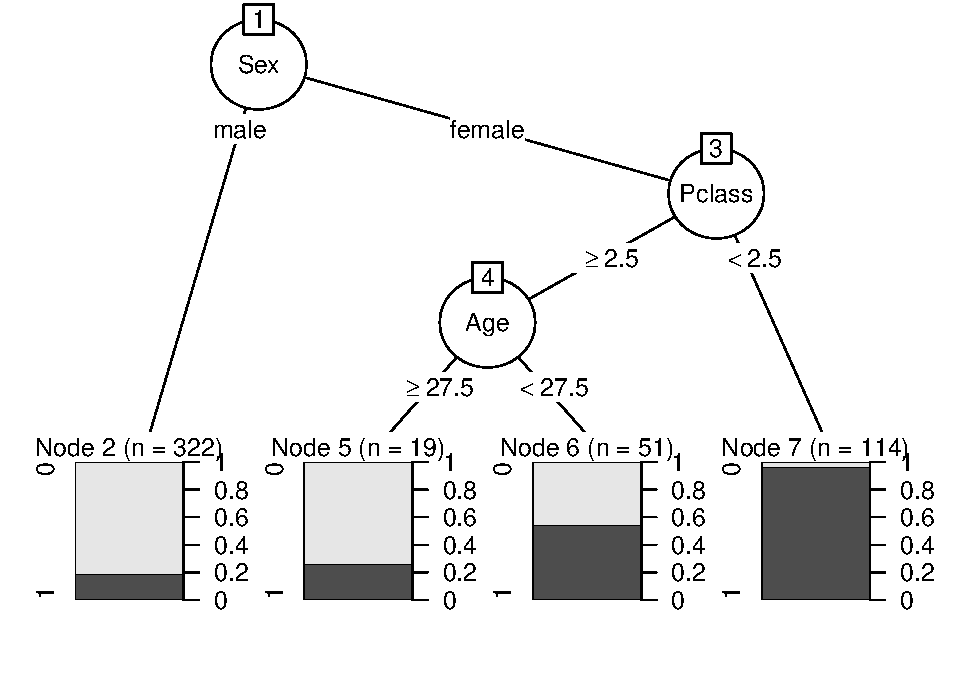
\includegraphics{homework_8_Hee_Bryan_files/figure-latex/unnamed-chunk-4-1.pdf}

\begin{Shaded}
\begin{Highlighting}[]
\NormalTok{test_tree6 <-}\StringTok{ }\KeywordTok{predict}\NormalTok{(tree_mod6, }\DataTypeTok{newdata =}\NormalTok{ Titanic_test2)[,}\DecValTok{2}\NormalTok{]}



\NormalTok{pred_logit6 <-}\StringTok{ }\KeywordTok{prediction}\NormalTok{(}\DataTypeTok{predictions =}\NormalTok{ test_logit6, }\DataTypeTok{labels =}\NormalTok{ Titanic_test2}\OperatorTok{$}\NormalTok{Survived)}
\NormalTok{pred_tree6 <-}\StringTok{ }\KeywordTok{prediction}\NormalTok{(}\DataTypeTok{predictions =}\NormalTok{ test_tree6, }\DataTypeTok{labels =}\NormalTok{ Titanic_test2}\OperatorTok{$}\NormalTok{Survived)}

\NormalTok{perf_logit6 <-}\StringTok{ }\KeywordTok{performance}\NormalTok{(pred_logit6, }\DataTypeTok{measure =} \StringTok{'tpr'}\NormalTok{, }\DataTypeTok{x.measure =} \StringTok{'fpr'}\NormalTok{)}
\NormalTok{perf_logit6_tbl <-}\StringTok{ }\KeywordTok{tibble}\NormalTok{(perf_logit6}\OperatorTok{@}\NormalTok{x.values[[}\DecValTok{1}\NormalTok{]], perf_logit6}\OperatorTok{@}\NormalTok{y.values[[}\DecValTok{1}\NormalTok{]])}
\KeywordTok{names}\NormalTok{(perf_logit6_tbl) <-}\StringTok{ }\KeywordTok{c}\NormalTok{(}\StringTok{'fpr'}\NormalTok{, }\StringTok{'tpr'}\NormalTok{)}

\NormalTok{perf_tree6 <-}\StringTok{ }\KeywordTok{performance}\NormalTok{(pred_tree6, }\DataTypeTok{measure =} \StringTok{'tpr'}\NormalTok{, }\DataTypeTok{x.measure =} \StringTok{'fpr'}\NormalTok{)}
\NormalTok{perf_tree6_tbl <-}\StringTok{ }\KeywordTok{tibble}\NormalTok{(perf_tree6}\OperatorTok{@}\NormalTok{x.values[[}\DecValTok{1}\NormalTok{]], perf_tree6}\OperatorTok{@}\NormalTok{y.values[[}\DecValTok{1}\NormalTok{]])}
\KeywordTok{names}\NormalTok{(perf_tree6_tbl) <-}\StringTok{ }\KeywordTok{c}\NormalTok{(}\StringTok{'fpr'}\NormalTok{, }\StringTok{'tpr'}\NormalTok{)}

\NormalTok{plot_roc <-}\StringTok{ }\ControlFlowTok{function}\NormalTok{(perf_tbl) \{}
\NormalTok{  p <-}\StringTok{ }\KeywordTok{ggplot}\NormalTok{(}\DataTypeTok{data =}\NormalTok{ perf_tbl, }\KeywordTok{aes}\NormalTok{(}\DataTypeTok{x =}\NormalTok{ fpr, }\DataTypeTok{y =}\NormalTok{ tpr)) }\OperatorTok{+}
\StringTok{  }\KeywordTok{geom_line}\NormalTok{(}\DataTypeTok{color =} \StringTok{'blue'}\NormalTok{) }\OperatorTok{+}
\StringTok{  }\KeywordTok{geom_abline}\NormalTok{(}\DataTypeTok{intercept =} \DecValTok{0}\NormalTok{, }\DataTypeTok{slope =} \DecValTok{1}\NormalTok{, }\DataTypeTok{lty =} \DecValTok{3}\NormalTok{) }\OperatorTok{+}
\StringTok{  }\KeywordTok{labs}\NormalTok{(}\DataTypeTok{x =} \StringTok{'False positive rate'}\NormalTok{, }\DataTypeTok{y =} \StringTok{'True positive rate'}\NormalTok{) }\OperatorTok{+}
\StringTok{  }\KeywordTok{theme_bw}\NormalTok{()}
  \KeywordTok{return}\NormalTok{(p)}
\NormalTok{\}}

\KeywordTok{plot_roc}\NormalTok{(perf_logit6_tbl)}
\end{Highlighting}
\end{Shaded}

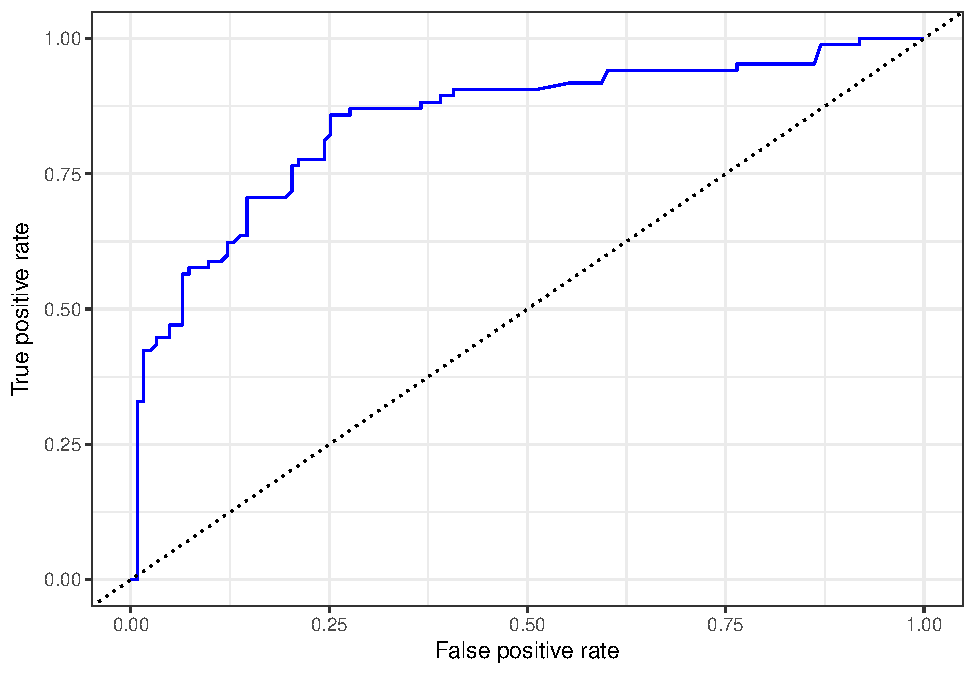
\includegraphics{homework_8_Hee_Bryan_files/figure-latex/unnamed-chunk-4-2.pdf}

\begin{Shaded}
\begin{Highlighting}[]
\KeywordTok{plot_roc}\NormalTok{(perf_tree6_tbl)}
\end{Highlighting}
\end{Shaded}

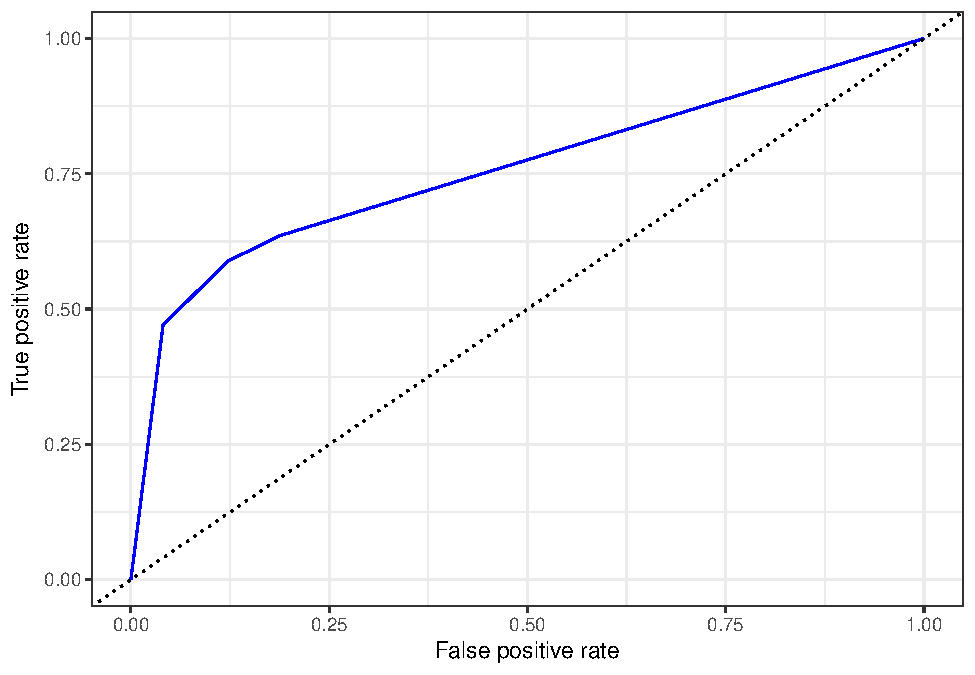
\includegraphics{homework_8_Hee_Bryan_files/figure-latex/unnamed-chunk-4-3.pdf}

\begin{Shaded}
\begin{Highlighting}[]
\NormalTok{auc_logit6 <-}\StringTok{ }\KeywordTok{performance}\NormalTok{(}\DataTypeTok{prediction.obj =}\NormalTok{ pred_logit6, }\DataTypeTok{measure =} \StringTok{"auc"}\NormalTok{)}
\NormalTok{auc_tree6 <-}\StringTok{ }\KeywordTok{performance}\NormalTok{(}\DataTypeTok{prediction.obj =}\NormalTok{ pred_tree6, }\DataTypeTok{measure =} \StringTok{"auc"}\NormalTok{)}

\CommentTok{# extract the AUC value}
\NormalTok{auc_logit6}\OperatorTok{@}\NormalTok{y.values[[}\DecValTok{1}\NormalTok{]]}
\end{Highlighting}
\end{Shaded}

\begin{verbatim}
## [1] 0.8472023
\end{verbatim}

\begin{Shaded}
\begin{Highlighting}[]
\NormalTok{auc_tree6}\OperatorTok{@}\NormalTok{y.values[[}\DecValTok{1}\NormalTok{]]}
\end{Highlighting}
\end{Shaded}

\begin{verbatim}
## [1] 0.7571497
\end{verbatim}

\begin{Shaded}
\begin{Highlighting}[]
\NormalTok{Titanic_test2 }\OperatorTok
\StringTok{  }\KeywordTok{mutate}\NormalTok{(}\DataTypeTok{pred_logit6 =}\NormalTok{ test_logit6,}
         \DataTypeTok{pred_tree6 =}\NormalTok{ test_tree6) ->}\StringTok{ }\NormalTok{Titanic_test2}

\NormalTok{cutoff =}\StringTok{ }\FloatTok{0.2}
\NormalTok{Titanic_test2 }\OperatorTok
\StringTok{  }\KeywordTok{mutate}\NormalTok{(}\DataTypeTok{logit6 =} \KeywordTok{case_when}\NormalTok{(pred_logit6 }\OperatorTok{>=}\StringTok{ }\NormalTok{cutoff }\OperatorTok{~}\StringTok{ "yes"}\NormalTok{,}
\NormalTok{                   pred_logit6 }\OperatorTok{<}\StringTok{ }\NormalTok{cutoff }\OperatorTok{~}\StringTok{ "no"}\NormalTok{), }
         \DataTypeTok{tree6 =}  \KeywordTok{case_when}\NormalTok{(pred_tree6 }\OperatorTok{>=}\StringTok{ }\NormalTok{cutoff }\OperatorTok{~}\StringTok{ "yes"}\NormalTok{,}
\NormalTok{                           pred_tree6 }\OperatorTok{<}\StringTok{ }\NormalTok{cutoff }\OperatorTok{~}\StringTok{ "no"}\NormalTok{)) ->}\StringTok{ }\NormalTok{Titanic_test2}


\NormalTok{Titanic_test2 }\OperatorTok\StringTok{ }\KeywordTok{count}\NormalTok{(logit6, Survived) }\OperatorTok\StringTok{ }\KeywordTok{spread}\NormalTok{(Survived, n)}
\end{Highlighting}
\end{Shaded}

\begin{verbatim}
## # A tibble: 2 x 3
##   logit6   `0`   `1`
## * <chr>  <int> <int>
## 1 no        76    10
## 2 yes       47    75
\end{verbatim}

\begin{Shaded}
\begin{Highlighting}[]
\NormalTok{Titanic_test2 }\OperatorTok\StringTok{ }\KeywordTok{count}\NormalTok{(tree6, Survived) }\OperatorTok\StringTok{ }\KeywordTok{spread}\NormalTok{(Survived, n)}
\end{Highlighting}
\end{Shaded}

\begin{verbatim}
## # A tibble: 2 x 3
##   tree6   `0`   `1`
## * <chr> <int> <int>
## 1 no      100    31
## 2 yes      23    54
\end{verbatim}


\end{document}
